\section{Background and Motivation}

%1. The appear of burst buffer
Burst buffer enabled IO architecture can help catch up with
the ever-increasing computational performance and parallelism of HPC system.
Burst buffer nodes debut as a rescue by utilizing various types of memory,
for example, non-volatile random-access memory (NVRAM) and solid state drive (SSD).
The driver behind is these storage technologies' decreasing cost of bandwidth.
In practice, it can suits up with DataWarp application I/O accelerator\cite{DataWarp}.
Figure \ref{Fig:BBArchitecture} illustrates one possible architecture of
burst buffer enabled HPC system, adopted by Trinity System\cite{TrinitySystem}.
%The volume of data read/write may affect the architecture model of burst buffer.
In Trinity, burst buffer nodes is composed of IO nodes and 2 PCIe SSD cards,
connected via totally 16 PCIe 3.0 interfaces.
Alternatively, many researchers proposed to distribute burst buffer 
on multiple layers of the memory hierarchy\cite{Romanus:CORR:15}.
For example, they may be deployed at local computer nodes, board in cabinet or IO nodes.
We may also use burst buffer as intermediate storage system.

\begin{figure*}[!t]
        \centering
        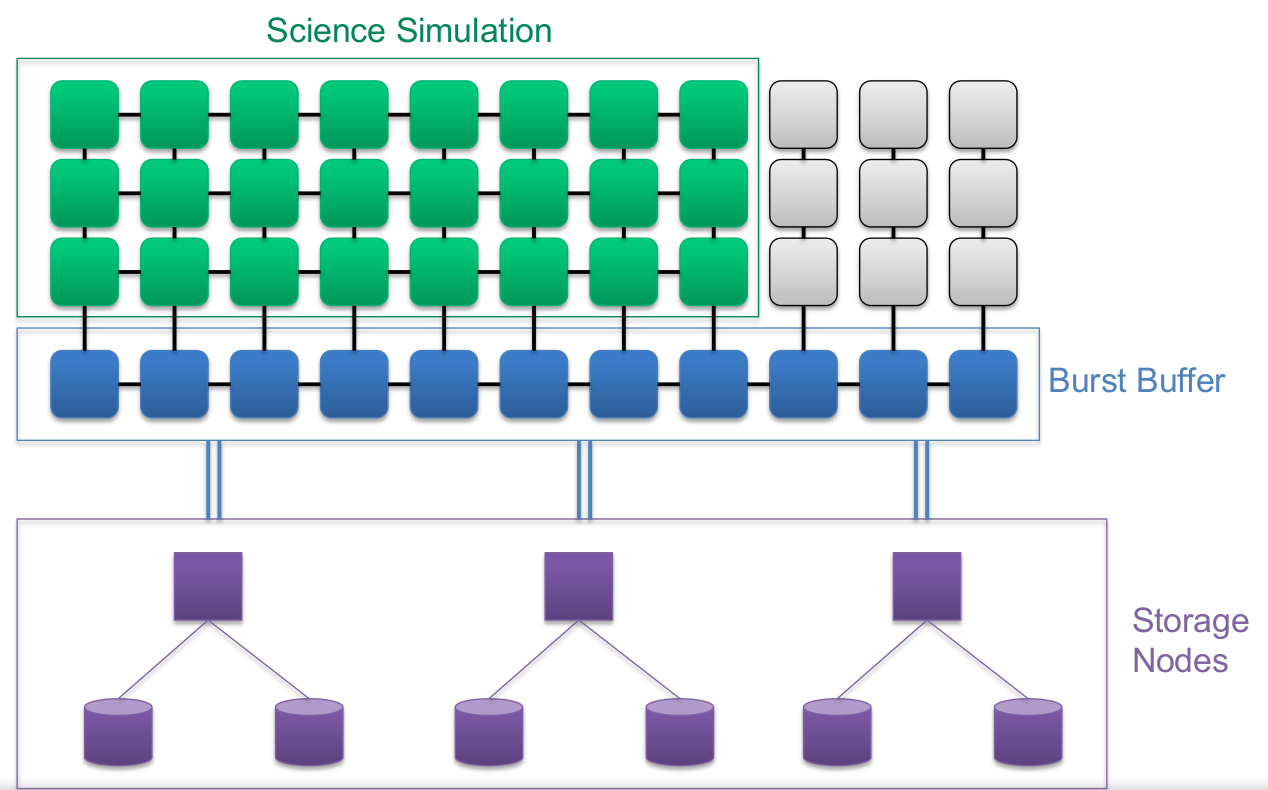
\includegraphics[width=6.6in]{BBArchitecture}
        \caption{Trinity System Overview: A Burst Buffer Enabled HPC System}
        \label{Fig:BBArchitecture}
\end{figure*}

%2. Use cases of burst buffer
Regardless of the specific implementation, burst buffer nodes essentially augment
the IO stack with a intermediate, productive offloading layer.
For example, an application's latest checkpoint can be pre-staged
before previous job terminates;
or an application can burst its checkpoint to burst buffer
with extremely high speed (4.4-17.8 TB/s on Trinity);
upon termination, application data is also able to drain off
asynchronously to external PFS.
When utilizing burst buffer in this primary scenario (\textit{checkpoint restart}),
bursty application IO operations can thus be aggregated and absorbed into burst buffers.
This makes it possible to shift computations that follows IO bursts to an earlier moment
while burst buffer takes charge of moving potentially TB-level volumes of data.
There are more use cases for burst buffer nodes.
Among them \textit{data cache} could be equally important to enhance the responsiveness
of applications by improving the perceived IO bandwidth\cite{BBUseCase}.
For example, shared object library or read-only configuration files could be
cached on burst buffer nodes;
lists of input files specific to a group of compute nodes allocated to
a particular application could be loaded to burst buffer prior to execution;
Economical solid-state disks as a tier of burst buffer could also be used as
out-of-core complement to insufficient main memory\cite{Romanus:CORR:15},
working place for data analysis (reductions, feature extraction compression etc.)
and visualization\cite{BBUseCase}.

%3. Motivate burst buffer aware scheduler
Given the critical role of burst buffer in future HPC IO system,
we expect user will be actively involved in requesting it for
better their own job's performance.
As a result, it is necessary, or even urgent, to systematically manage
the allocation of these second precious resources (secondary to compute nodes).
This naturally falls into the responsibility of HPC workload scheduler.
Unfortunately, existing schedulers
either have not yet been aware to burst buffer\cite{Moab} %other scheduler citation needed
or just provide very naive allocation policy\cite{SlurmBBGuide}.
This paper tries to bridge two isolated fields of HPC architecture,
the novel burst buffer equipped HPC IO subsystem and
traditional batch job queueing subsystem.
The bridge build upon a 3-phase model that motivated by two of the most
important usage cases of burst buffer:
application checkpoint restart and data cache/pre-fetch for stage in/out.
The benefit of burst buffer nodes will be more than just higher transfer
bandwidth, if it were intelligently allocated by scheduler.
For example, the first case could speedups the \textit{running phase} of
user's application by acutely absorb the bursty checkpoint-purpose IO request;
the second case reduce the application's waiting time via
contracted input/output stage in the execution pipeline of application series.

%4. Contribution summary and paper structure
Our contributions in this paper are summarized as follows:
\begin{enumerate}
        \item Explore how HPC workload scheduler allocates burst buffer resources.
                We propose a 3-phase application model tailored the typical
                usage scenarios of burst buffer, that is, checkpoint restart,
                data file/cache stage in and stage out.
        \item On the basis of 3-phase job model, we present Cerberus,
                a burst buffer aware HPC workload scheduler.
                Dividing the lifetime of user application to different phases,
                Cerberus makes it possible to conquer the scheduling goal separately.
        \item We suggest several optimizing goals for each phases.
                Though optimal scheduling problem in each phase is NP-hard,
                dynamic programming with memoization could give precise solutions
                in practice.
\end{enumerate}

In the reminder of this paper,
the next section begins elaborating the 3-phase model (section~\ref{Sec:Model}),
after which Cerberus is introduced in section~\ref{Sec:Scheduler}.
The details of formulating and solving scheduling problems with
dynamic programming at each job phase are also
enumerated in section~\ref{Sec:Scheduler}.
Starting from section~\ref{Sec:Experiments}, we validate Cerberus
by simulating the full Trinity supercomputing platform, featured with
burst buffer hardware.
Related works are discussed in section~\ref{Sec:RelatedWorks}.
We conclude this paper and list possible future works in section~\ref{Sec:Conclusion}.


